\section{Background and Motivation}
\label{background}

Artificial Intelligence (AI) is one of the fastest growing technology domains, involving academic research, businesses, and users. 
The enormous investment in AI led to groundbreaking applications in a diverse set of areas.  AI is used for accelerating the discovery of
drugs (~\cite{stark2022equibind}), driving efficiencies at work (e.g.,~\cite{puri2021codenet}), discovering new materials towards renewable storage (e.g.,~\cite{zitnick2020}), and more. 
\cite{Rous08}
%While there is no doubt about the enormous potential of AI to 
%change the way we live, 
%we are also in the midst of a heated debate about the potential of AI to harm (e.g., 
%\cite{aidanger}m ~\cite{godfather}). Risks frequently associated with AI include, fake news, biases, job losses, and, huge environmental cost. 
%%
%Multiple researchers and practitioners have raised the alarm on the environmental cost of AI, and offered a calls-to-action (\cite{Strubell2019, Lacosta2019, Henderson2020, Bender2021, paterson2021}. For example, it is shown (\cite{Strubell2019}) that training a single large transformer model on a GPU device, can take up to the equivalent carbon of $5$ cars
%through their entire life time. The amount of compute used to train deep learning models has increased $300,000\times$ in six years~\cite{schwartz2019green}. 
%Data has increased significantly in the last two years, reaching exabyte scale. The data size increase has led to a $3.2\times$ increase in the data ingestion bandwidth demand~\cite{ml-sys22}. The ever-increasing data volume has driven a super-linear trend in model size growth. We are witnessing $1000\times$ model size increase for $GPT3$ based language translation tasks (\cite{brown2020language}). Amidst the exponential growth in data and models, systems capacity only grew moderately. The memory capacity of GPU-based accelerators, e.g. $32GB$ (NVIDIA V100, 2018) to $80GB$ (NVIDIA A100, 2021), has increased by $< 2\times$ every $2$ years. The resource requirements for strong AI scaling clearly outpaces that of system hardware, which has motivated a 
%variety of scale-out infrastructure solutions (e.g.,~\cite{patterson2021carbon}). 
%
%Another fascinating trend, is the emergence of Foundation Models~\cite{fm-stanford},  which are trained on very broad data using self supervision at scale. One of the interesting characteristics of Foundation Models is that 
%through the concept of transfer learning (~\cite{thrun1998lifelong})
%they can be adapted (e.g., fine-tuned, or distilled) to a wide range of downstream tasks.  In fact, the majority of state-of- the-art NLP models are now adapted from one of a few foundation models, such as BERT (~\cite{devlin2018bert}), RoBERTa (~\cite{liu2019roberta}), BART (~\cite{lewis2019bart}), T5 (~\cite{raffel2020exploring}) etc. 
%Foundation models are not new, but the scale, scope, and emergent capabilities of foundation models in the last few years have exceeded our imagination. For example, GPT-3 has $175$ billion parameters (in comparison with the 'modest' 1.5 billion parameters of its predecessor GPT-2) and can be adapted via natural language prompts to perform a range of tasks despite not being trained explicitly to do many of those tasks~\cite{brown2020}. 
%
%In this position paper, we apply knowledge of sustainability principles, protocols and standards
%including the GHG Protocol~\cite{}, and product Life Cycle Assessment (LCA)~\cite{})
%to the area of AI in order to develop metrics that can be meaningfully used to drive sustainability mind-set and examine trade-offs across the life cycle of 
%AI models. Defenders of Foundation Models often claim that while the up-front environmental cost of training a Foundation Model 
%is enormous, because they promote  low cost re-use at scale they contribute to reducing the overall global cost of AI. In order to analytically tackle this question, our metrics definition factors-in the entire 'supply chain' of models in defining the amortized cost of the actual unit of work performed, namely, the inference jobs submitted by end-user. 
%We believe that this approach can  enable a more meaningful debate and selection of strategies ultimately leading to environmental harm reduction. 
%Our goal in this paper is to define metrics that can be used to evaluate AI efficiency {\em end-to-end} focusing on the end-user inference jobs as the main entity of interest and factoring in the entire 'supply chain' of models. We associating operational and embodied sustainability cost with end user driven inference jobs.
%
%We base our work on the recent HotCarbon paper ``Metrics for Sustainability in DC" (~\cite{}), that defines metric for sustainability costs in a data center in the granularity of a unit of work, produced on behalf of an end user, termed, {\em a job}. We follow the same design principles, aiming at metrics that will incentivize end-users and  data-scientists, towards a sustainability mind-set, using metrics that are measurable easy to calculate, reproducible, and useful. We have made efforts to re-use the metrics defined in~\cite{}, specifically, Job Sustainability Cost (JCS), and Amortized Sustainability Cost (ASC). Unfortunately, in our analysis, we reached a conclusion that one component is missing from the metrics definition; which is, the cost of any software asset that is serving as the context of the execution of the job being evaluated. 
%Examples of 'software asset' include, an always running platform service that is supporting the execution of a job, such as, the Lambda service~\cite{} for Serverless jobs in AWS~\cite{}, or 
%an AI model that is used for inference jobs.
%In both cases, there is not only a significant operational overhead
%to maintain the assets, (such as health, and continuous development of an on-line platform service, or, continuous re-train of a model to maintain accuracy), there is also what we call 'embodied' cost of software, which we adopt from its use for IT systems to capture the energy and carbon cost to develop and test the software asset (such as platform development, or, model training). 
%The contribution of our paper is as follows: 
%\begin{enumerate}
%    \item We define a new metric {\em Embodied Product Cost}, that aims at expressing the 'embodied' carbon of software assets,  i.e., the carbon cost of 'manufacturing' a software asset, such as the development and testing of an on-line platform, or the up-front training of an AI model. 
%    \item we expand the definitions of Job Sustainability Cost, and 
%    Amortized Sustainability cost, defined in~\cite{} to factor-in the operational cost of the software asset used as the
%    context of the execution of the job, as well as, the 'embodied' costs of these software assets.
%    \item we specialize and apply these new metrics to the case of AI. We show how our approach can promote a sustainability mind-set, and in particular can be used (for the first time, to the best
%    of our knowledge) to analytically prove or refute the claim that foundations model re-use for downstream tasks is advantageous to the environment, relative to the construction of smaller more specific models, from scratch.
%    \item using the new metrics, we analyse the new opportunities for sustainability based research across the life-cycle of models, Such as life-cycle strategies (e.g., use of Neural Architecture Search, or frequency of re-training, or re-use benefits), and 
%    trade-offs, based on requirements and expected use. 
%\end{enumerate}
%
%\subsection{Related Work}
%
%> sustainable computing -- measuring, other standards - no more paragraph (EK)
%> sustainable ai - MEta, FB, Green AI, Stadler? bruno - mo more pararaph (Tamar)
%> ai optimization which is not energy related (bhatta)
%
%NOTES:
%Summary of limitations of current approaches
%- A single total number for energy and carbon footprint throughout the life cycle of the model such as in ~\cite{https://arxiv.org/abs/2104.10350} is not meaningful. It gives a total number which does not correspond to efficiency because it does not factor in the amount of work being done. In addition, It does not factor in the on-going maintenance of the model, e.g., re-training. 
%- System quantification such as energy for processing a single round(?) is useful to compare different systems such as A100 vs V100 but does not give the full picture, since efficiency improvement is also achieved in the algorithmic level thus reducing the number of rounds required
%- Meta paper {} consider all phases of life cycle in isolation however it does not factor in the amount of work performed (number of transactions), and cannot be used to compare strategies (for example re-use vs from scratch) without additional work Bruno's paper - only training 
%%% to-do: Review existing work - GreenAI paper, Meta paper, Google Paper, Strubel, etc. and their limitations. 
%
%\begin{itemize}
%\item sustainable AI \cite{Wu2022}
%\item datacenter decarbonization \cite{Chien2022,Acun2023,Maji2022}
%\item AI model optimization \cite{Patterson2022,Frey2022,Qiao2021,Li2016}
%\item datacenter optimization \cite{Souza2022,Townend2019}
%\item datacenter thermal \cite{Chi2020,Li2020,Tian2020,Ilager2019,Linder2019,Acun2017}
%\item hpc energy \cite{Tracey2020}
%\end{itemize}
%
%\subsection{The life cycle of an AI model}
%%% Introduce Foundation Models,  what are they and why we ought to think differently about 
%%% the life cycle efficiency - how do we factor in re-use, model distelation, fine-tuning, and re-training? 
% %% Describe the model life cycle in details - all the stages ****plus a working example****
%A foundation model is a large artificial intelligence model trained on a vast quantity of data at scale (often by self-supervised learning or semi-supervised learning) resulting in a model that can be adapted to a wide range of downstream tasks ~\cite{}. 
%A majority of NLP models are now developed based on  a few foundation models, such as BERT, RoBERTa, BART, or, T5. It is projected ~\cite{} that foundation models will be developed across a wide range of modalities.
%
% To fully understand the real environmental impact, and be able to assess the impact and develop the appropriate metrics
% we must first of all take a close look at a model life cycle, end-to-end, including: data collection, model exploration and experimentation, model training, model distillation, and fine tuning, deployment, and then re-training, and inference cost. 
%%% \begin{figure*}[t]
%%%\centerline{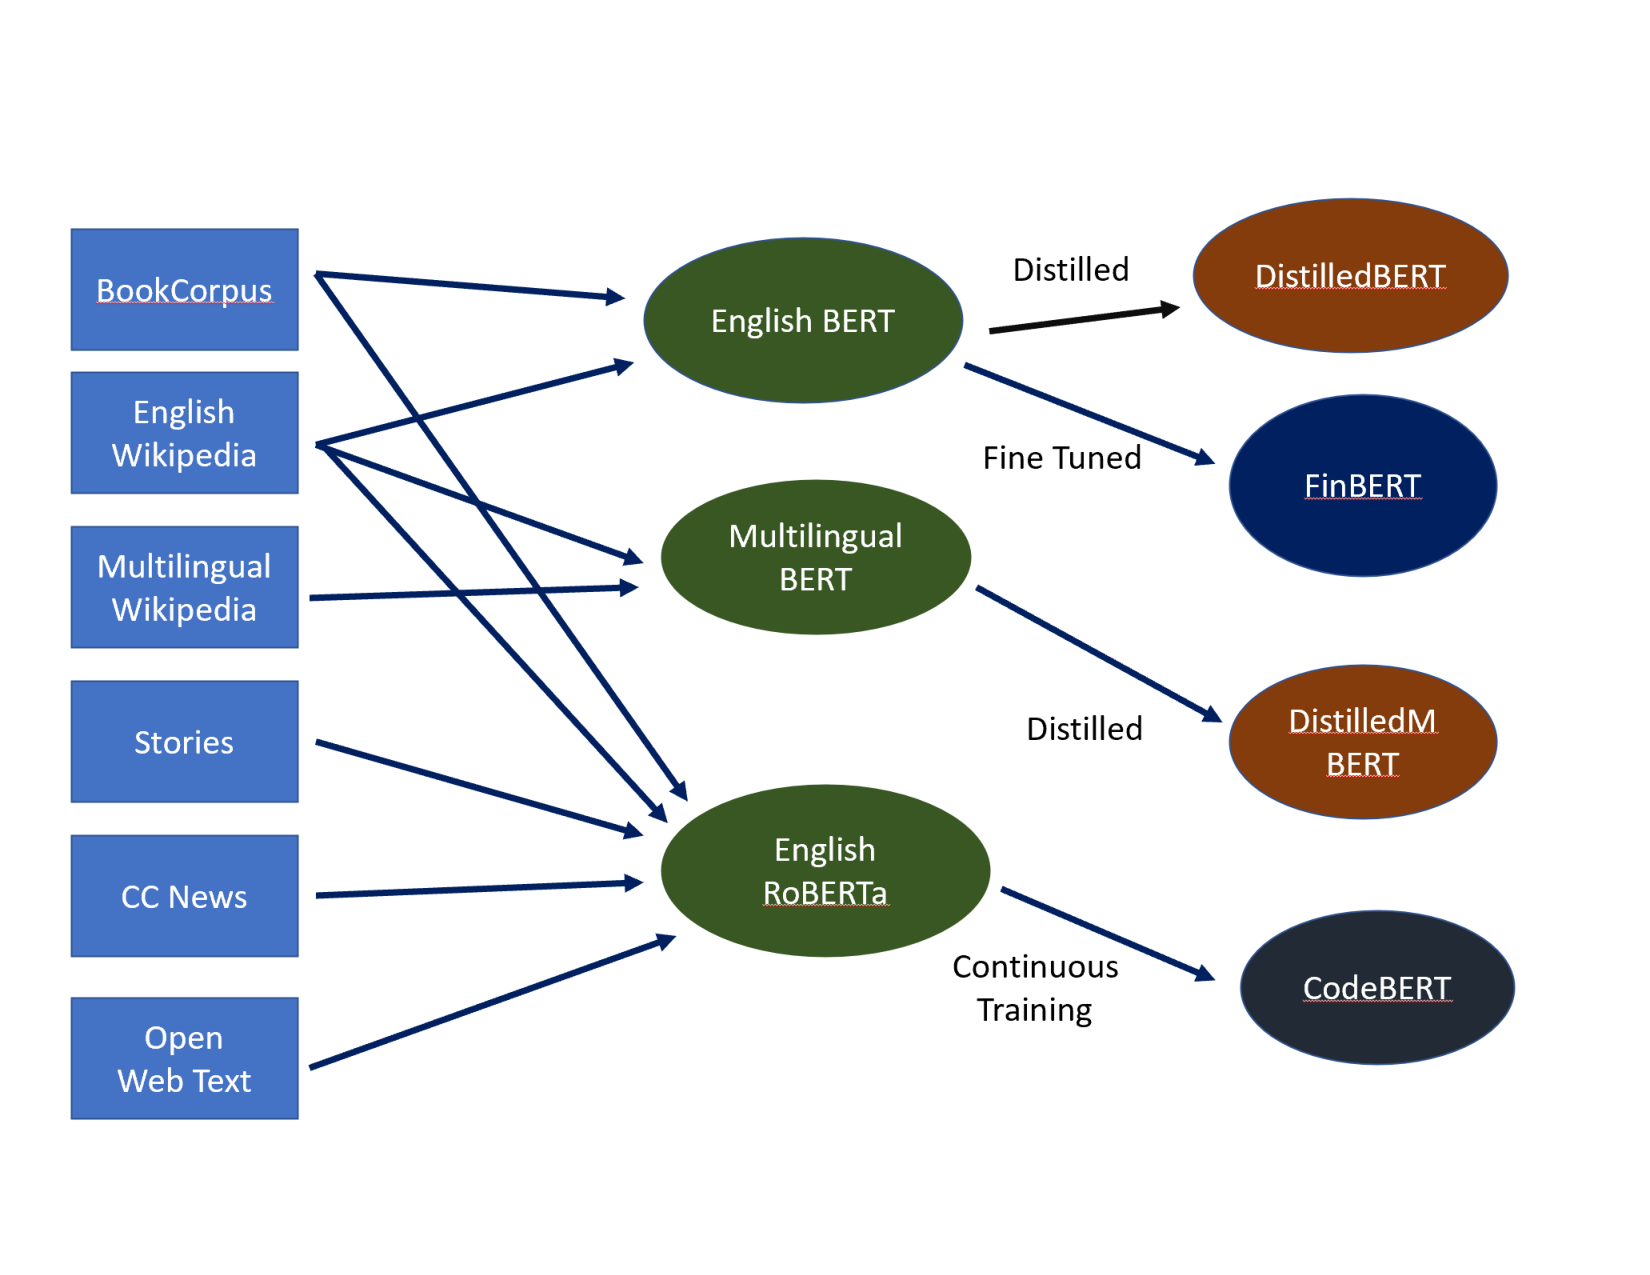
\includegraphics[width=8cm]{model-2.pdf}}
%%%\caption{The 'Supply Chain' of data-sets and models}
%%%  \label{fig:model-life-cycle}
%%%\end{figure*}
%
%\begin{figure}[]
%\centering{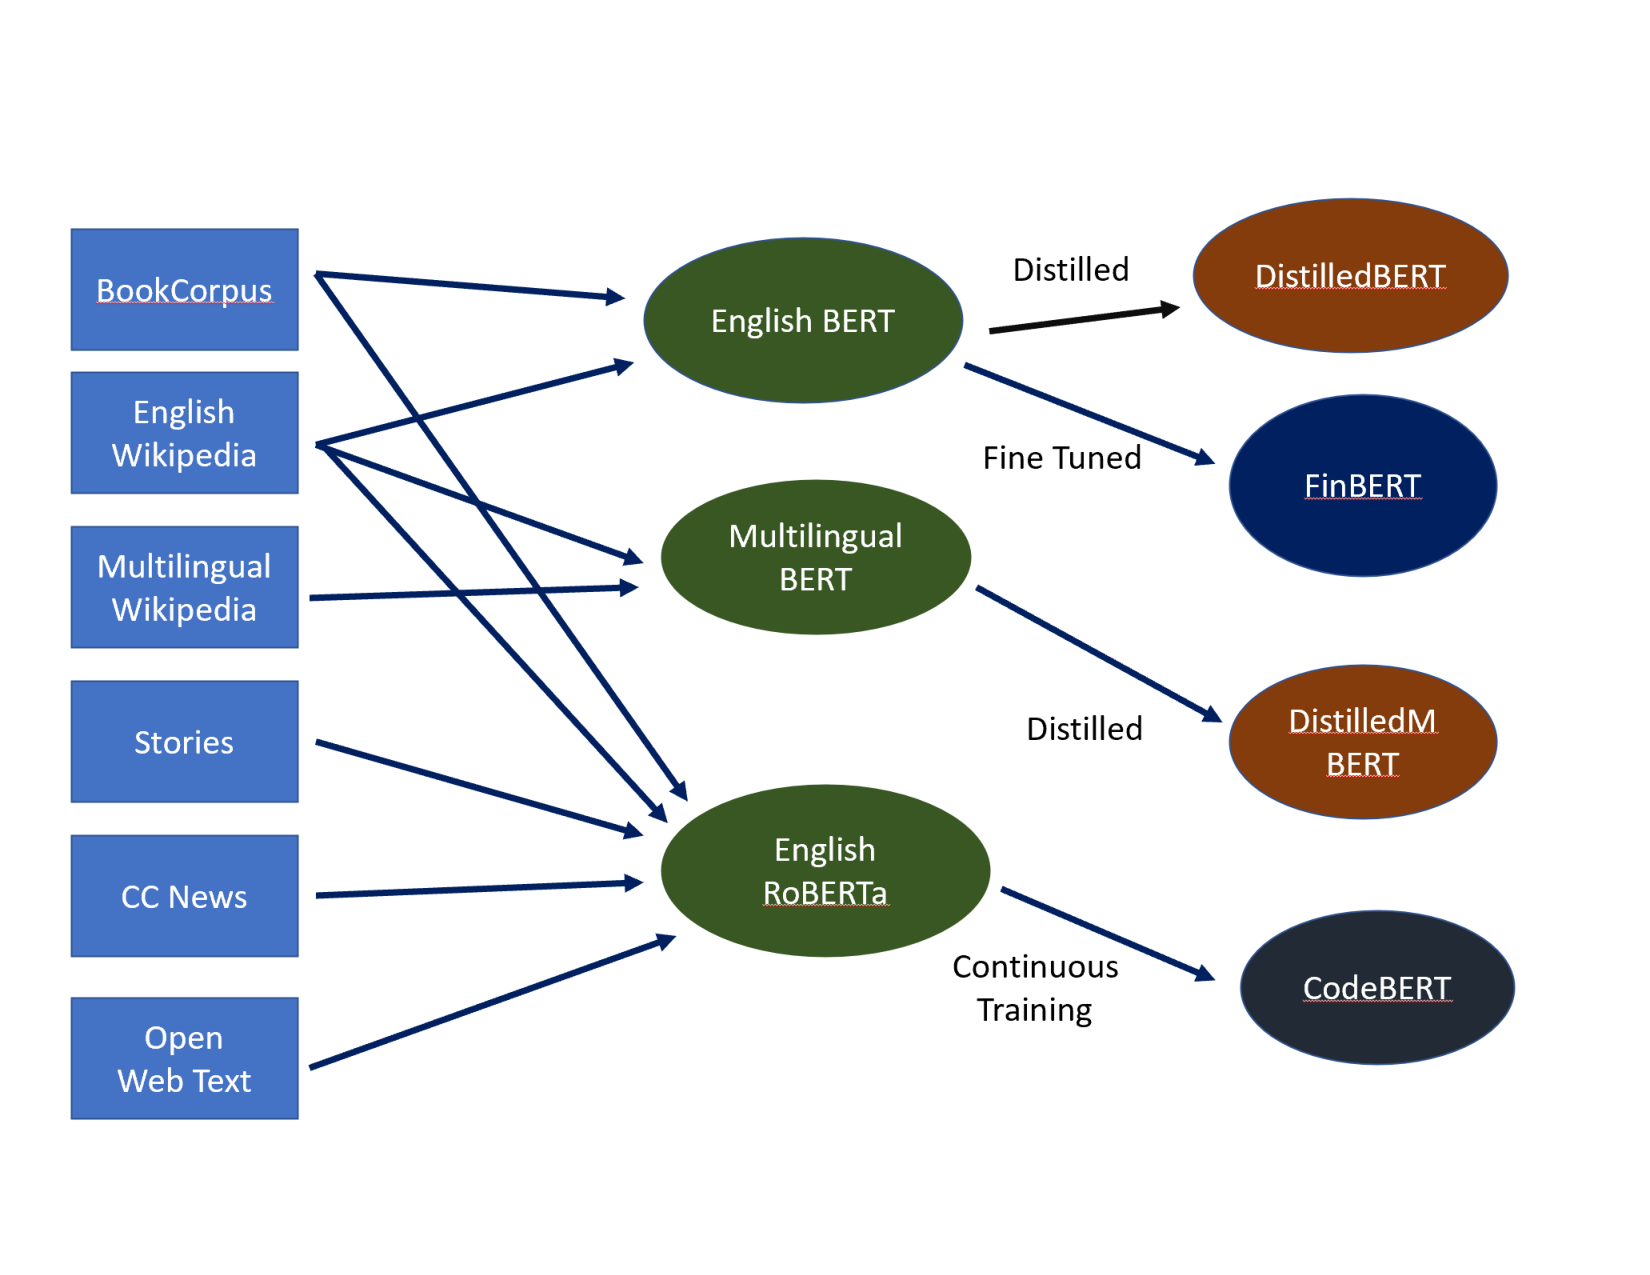
\includegraphics[width=8cm]{model-2.pdf}}
%\caption{The 'Supply Chain' of data-sets and models}
%  \label{fig:model-life-cycle}
%\end{figure}
%
%A pre-processing pipeline needed to curate data for training a model could consist of the following steps: Data acquisition:  Via crawling (for NLP) or running simulations (materials or physics); De-duplicating:  To ensure there Is one copy of a document from multiple sources; Selecting documents of certain languages of interest; Splitting the documents into sentences for training; Identifying Hate Abuse Profanity and PII information one may want to filter; Forming the data files for training based on a format
%For example, NLP datasets such as  Wikipedia,  Stories,  OpenWebText, BookCorpus, CC News which are constructed via web crawling. 
%Each of them could potentially be processed through all the above steps before it is ready for being used for training.  Fig \ref{fig:model-preprocess} shows such a pipeline
% 
% \begin{figure}[]
%\centering{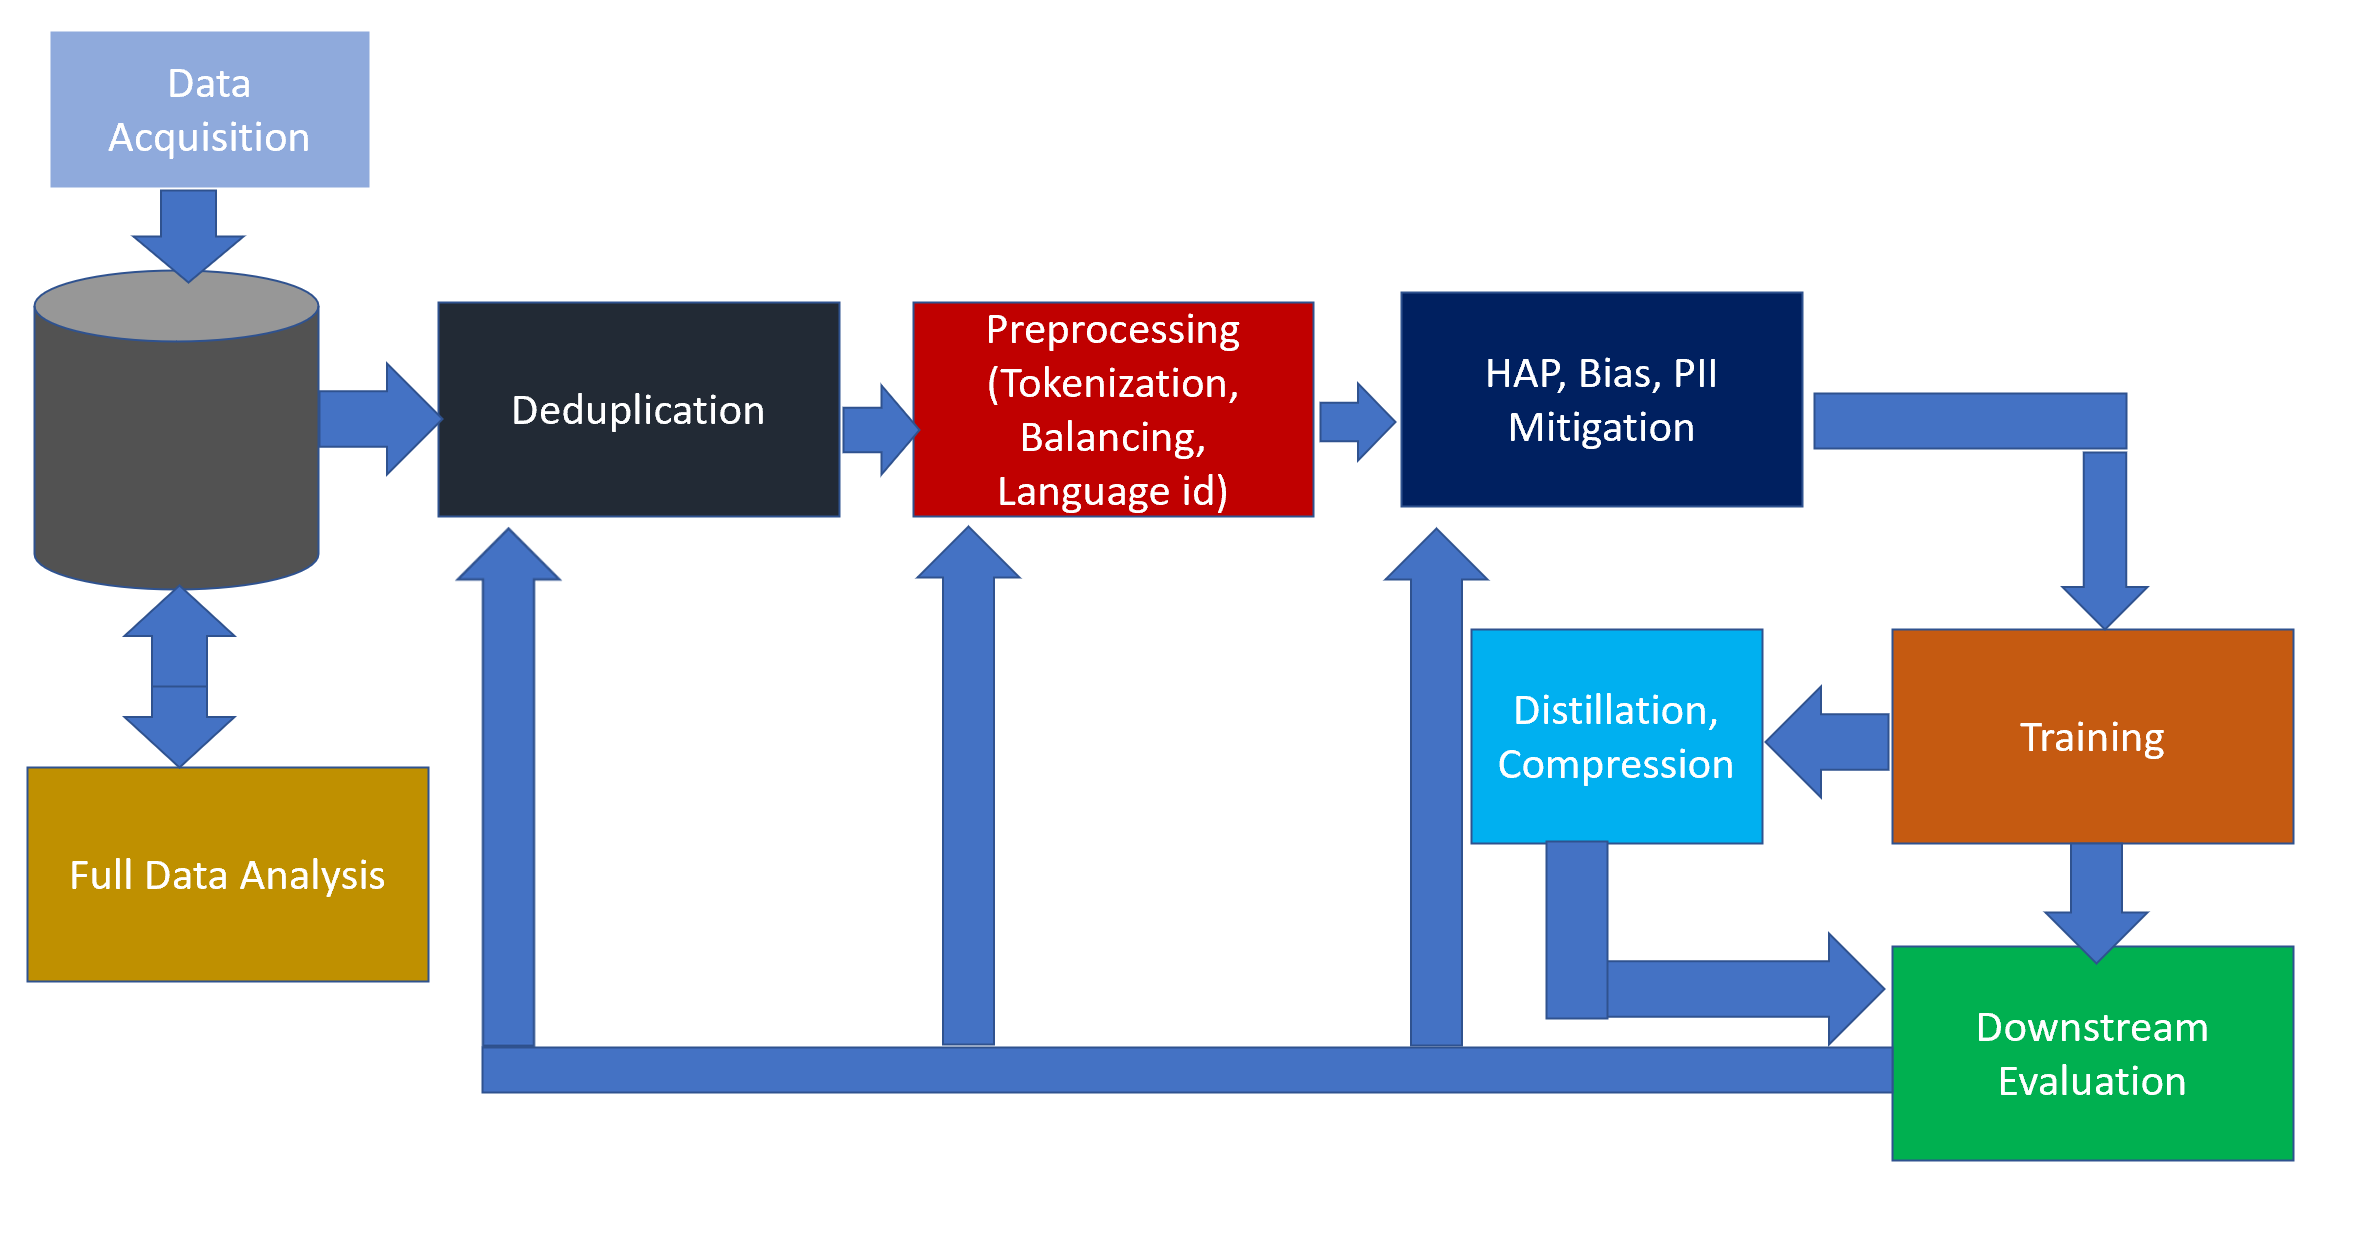
\includegraphics[width=8cm]{sustain3.png}}
%\caption{A typical preprocessing pipeline}
%  \label{fig:model-preprocess}
%\end{figure}
%
%
%These datasets have been used to train multiple models in various combinations.  BERT was trained using English Wikipedia and BookCorpus.  Whereas Multilingual BERT (mBERT) was trained on multilingual Wikipedia over 100+ languages.   RoBERTa on English data-sets spanning Wikipedia, Stories, OpenWebText, BoockCorpus as well as CC-News.  
%%The effort needed to curate this datasets gets amortized over multiple models which benefit from it in various proportions - will get to this later
%After a model is trained, the model may be distilled to bring it to a form factor which fits certain latency or space budget. For example  DistilBERT and DistilMBERT are based on BERT and mBERT respectively.  They are of 6 layers instead of the 12 layers in BERT and has $40\%$ less parameters then BERT base uncased; it runs $60\%$ faster while preserving $95\%$ pf the accuracy of BERT base on GLUE benchmark.
%
%The base model could also be further finetuned or  continuously trained for a certain domain. FinBERT was created by finetuning a BERT model on finance data and CodeBERT was created by continuously training RoBERTa over github repositories. FinBERT delivers better result than the base BERT on financial analysis benchmarks like FiQA Sentiment Scoring and Financial Phrasebank. There is some additional effort needed for fine-tuning and continuous training to produce these models.
%The effort needed to create the BERT base is now not only utilized when BERT is used directly on any task but also when models spun off from it are also utilized.
